% SPDX-License-Identifier: PMPL-1.0-or-later
% SPDX-FileCopyrightText: 2026 Jonathan D.A. Jewell
%
% Economics-as-Code: Shadow Pricing, Carbon-Aware Execution, and
% Multi-Objective Resource Optimization in Programming Language Design
%
% arXiv preprint — Eclexia programming language

\documentclass[11pt,a4paper]{article}

% --- Packages ---
\usepackage[utf8]{inputenc}
\usepackage[T1]{fontenc}
\usepackage{amsmath,amssymb,amsthm}
\usepackage{mathtools}
\usepackage{stmaryrd}
\usepackage{listings}
\usepackage{xcolor}
\usepackage{hyperref}
\usepackage{cleveref}
\usepackage{booktabs}
\usepackage{multirow}
\usepackage{graphicx}
\usepackage{algorithm}
\usepackage{algpseudocode}
\usepackage{tikz}
\usetikzlibrary{arrows.meta,positioning,shapes.geometric,calc}
\usepackage{pgfplots}
\pgfplotsset{compat=1.18}
\usepackage[margin=1in]{geometry}
\usepackage{microtype}
\usepackage{enumitem}
\usepackage{subcaption}
\usepackage{fancyhdr}

% --- Theorem environments ---
\newtheorem{theorem}{Theorem}[section]
\newtheorem{lemma}[theorem]{Lemma}
\newtheorem{proposition}[theorem]{Proposition}
\newtheorem{corollary}[theorem]{Corollary}
\newtheorem{definition}[theorem]{Definition}
\newtheorem{example}[theorem]{Example}
\newtheorem{remark}[theorem]{Remark}

% --- Listings configuration ---
\definecolor{eclkw}{HTML}{7B2D8B}
\definecolor{eclann}{HTML}{C05000}
\definecolor{eclstr}{HTML}{2E7D32}
\definecolor{eclcmt}{HTML}{6A737D}
\definecolor{eclnum}{HTML}{0D47A1}
\definecolor{eclbg}{HTML}{F8F8F8}

\lstdefinelanguage{Eclexia}{
  keywords={def, fn, adaptive, let, if, else, while, for, in, return, type, struct, enum, match, impl, trait, pub, mod, use, spawn, channel, send, recv, select, yield, assert, true, false},
  keywordstyle=\color{eclkw}\bfseries,
  sensitive=true,
  comment=[l]{//},
  morecomment=[s]{/*}{*/},
  commentstyle=\color{eclcmt}\itshape,
  stringstyle=\color{eclstr},
  morestring=[b]",
  moredelim=[is][\color{eclann}\bfseries]{@}{:},
  moredelim=[is][\color{eclann}\bfseries]{@}{\ },
  literate={->}{$\rightarrow$}2 {<}{$<$}1 {>}{$>$}1,
  numbers=left,
  numberstyle=\tiny\color{gray},
  numbersep=5pt,
  basicstyle=\ttfamily\small,
  backgroundcolor=\color{eclbg},
  frame=single,
  framerule=0.4pt,
  xleftmargin=2em,
  framexleftmargin=1.5em,
  breaklines=true,
  tabsize=4,
  showstringspaces=false,
}

\lstset{language=Eclexia}

% --- Math operators ---
\DeclareMathOperator*{\argmin}{arg\,min}
\DeclareMathOperator*{\argmax}{arg\,max}
\DeclareMathOperator{\cost}{cost}
\DeclareMathOperator{\feasible}{feasible}
\DeclareMathOperator{\shadow}{shadow}
\DeclareMathOperator{\carbon}{carbon}
\DeclareMathOperator{\energy}{energy}
\DeclareMathOperator{\minimize}{minimize}
\DeclareMathOperator{\maximize}{maximize}

% --- Title ---
\title{%
  \textbf{Economics-as-Code: Shadow Pricing, Carbon-Aware Execution, and
  Multi-Objective Resource Optimization in Programming Language Design}
}

\author{%
  Jonathan D.A. Jewell \\
  \texttt{j.d.a.jewell@open.ac.uk} \\
  \url{https://github.com/hyperpolymath}
}

\date{March 2026}

% --- Document ---
\begin{document}

\maketitle

% ============================================================
% ABSTRACT
% ============================================================
\begin{abstract}
Software systems consume approximately 4\% of global electricity and are
responsible for a growing share of greenhouse gas emissions, yet mainstream
programming languages treat energy, carbon, and time as invisible externalities.
We present \textsc{Eclexia}, a programming language that elevates resource
constraints---energy, time, memory, and carbon---to first-class citizens in the
type system.  Functions declare resource requirements via \texttt{@requires} and
\texttt{@provides} annotations that are verified at compile time and enforced at
runtime.  A novel \emph{shadow pricing} mechanism, grounded in the duality
theory of linear programming, assigns implicit prices to scarce resources and
guides the runtime in selecting among \emph{adaptive function solutions}---multiple
implementations of the same function that form a Pareto frontier over
multi-objective resource costs.  The runtime further integrates real-time
electricity grid carbon intensity data, enabling \emph{carbon-aware execution}
that temporally shifts heavy computation to low-carbon periods.  We formalize
the core calculus $\lambda^{\mathrm{ecl}}$ and prove type safety, resource
safety, and monotonicity of shadow prices.  Resource bound proofs are
mechanizable via Coq and Agda backends.  Our prototype compiler, implemented in
Rust, targets a stack-based bytecode VM, WebAssembly, and LLVM IR.
Preliminary evaluation on representative workloads shows $23$--$61\%$
energy savings and $31$--$74\%$ carbon reduction compared to
resource-oblivious baselines, with negligible runtime overhead ($<2\%$) for
shadow price computation.  Eclexia demonstrates that sustainability need not be
an afterthought---it can be a first-class language design principle.

\medskip
\noindent
\textbf{Keywords:} resource-aware programming languages, shadow pricing,
carbon-aware computing, multi-objective optimization, adaptive execution,
sustainable software engineering, type systems
\end{abstract}


% ============================================================
% 1. INTRODUCTION
% ============================================================
\section{Introduction}
\label{sec:introduction}

\subsection{The Hidden Costs of Computation}

The global information and communications technology (ICT) sector consumed an
estimated 1,500--2,000\,TWh of electricity in 2024, a figure projected to reach
3,000\,TWh by 2030 under current growth trajectories~\cite{jones2018,
masanet2020}.  Data centers alone account for roughly 1--1.5\% of global
electricity demand, and the rapid expansion of machine learning workloads is
accelerating this trend.  Yet the programming languages in which nearly all of
this software is written---C, Java, Python, JavaScript, Rust, Go---are
fundamentally \emph{resource-oblivious}.  They provide no language-level
abstraction for reasoning about energy consumption, carbon emissions, memory
pressure, or real-time cost.

This obliviousness has consequences.  A function that performs matrix
multiplication consumes the same energy whether the device is plugged into
hydroelectric power or a diesel generator.  A cloud service processes requests
identically whether electricity costs \$0.02/kWh or \$0.40/kWh.  A mobile
application drains its battery at the same rate whether the user has 80\% charge
remaining or 3\%.

We argue that this disconnect between computation and its physical costs is not
merely an engineering oversight---it is a \emph{design failure} in programming
language theory.  The type systems we have built are extraordinarily
sophisticated at tracking data flow, ownership, and concurrency, yet remain
silent on the most consequential dimension of modern software: its environmental
and economic footprint.

\subsection{The Case for Economics-as-Code}

We propose a paradigm we call \emph{economics-as-code}: the integration of
resource economics directly into the semantics of a programming language.  In
this paradigm:

\begin{enumerate}[label=(\roman*)]
  \item \textbf{Resource constraints are types.}  Functions carry
    \texttt{@requires} and \texttt{@provides} annotations that declare energy,
    time, memory, and carbon budgets.  The compiler reasons about these
    annotations using constraint propagation and abstract interpretation.

  \item \textbf{Shadow prices guide execution.}  Every resource has a
    dynamically-updated \emph{shadow price} reflecting its current scarcity.
    The runtime uses these prices to make locally optimal decisions via the
    weighted-cost objective $\sum_r \lambda_r \cdot p_i(r)$, where $\lambda_r$
    is the shadow price of resource $r$ and $p_i(r)$ is the resource profile
    of solution $i$.

  \item \textbf{Functions are adaptive.}  A single function signature may have
    multiple implementations (\emph{solutions}).  The runtime selects the
    Pareto-optimal solution given current constraints and shadow prices.

  \item \textbf{Carbon is a first-class resource.}  The runtime queries
    real-time grid carbon intensity and incorporates it into scheduling
    decisions, enabling temporal shifting of computation to low-carbon periods.
\end{enumerate}

\subsection{Contributions}

This paper makes the following contributions:

\begin{itemize}
  \item The design and formalization of the core calculus $\lambda^{\mathrm{ecl}}$,
    a typed lambda calculus extended with resource annotations, adaptive blocks,
    and shadow pricing (\cref{sec:type-system,sec:shadow-pricing}).

  \item A formal model of shadow pricing grounded in LP duality theory, with
    proofs of non-negativity, monotonicity, and convergence
    (\cref{sec:shadow-pricing}).

  \item An adaptive function selection mechanism based on multi-objective Pareto
    optimization over (time, energy, memory, carbon)
    (\cref{sec:adaptive-functions}).

  \item A carbon-aware scheduling algorithm that integrates real-time grid
    data with a competitive ratio of at most~2 (\cref{sec:carbon-scheduling}).

  \item A prototype implementation in Rust with three backends (bytecode VM,
    WASM, LLVM IR) and preliminary evaluation (\cref{sec:implementation,sec:evaluation}).

  \item Mechanized proofs of type safety and resource safety in Coq and Agda
    (\cref{sec:formal-verification}).
\end{itemize}

\subsection{Paper Organization}

\Cref{sec:background} surveys relevant background.
\Cref{sec:type-system} presents the resource annotation system and type rules.
\Cref{sec:shadow-pricing} formalizes the shadow pricing model.
\Cref{sec:adaptive-functions} describes adaptive function selection.
\Cref{sec:carbon-scheduling} covers carbon-aware scheduling.
\Cref{sec:formal-verification} addresses formal verification.
\Cref{sec:implementation} details the implementation.
\Cref{sec:evaluation} presents our evaluation.
\Cref{sec:related-work} discusses related work.
\Cref{sec:discussion} reflects on implications.
\Cref{sec:conclusion} concludes.


% ============================================================
% 2. BACKGROUND
% ============================================================
\section{Background}
\label{sec:background}

\subsection{Resource-Aware Compilation}

The idea of tracking resources at the language level has a long history.
Hofmann and Jost~\cite{hofmann2003} introduced \emph{automatic amortized resource
analysis} (AARA), which infers polynomial resource bounds via a type system
augmented with potential annotations.  The Resource Aware ML (RaML)
system~\cite{hoffmann2012} extended this to higher-order programs with
multivariate polynomial bounds.  These systems focus primarily on heap space;
Eclexia generalizes the approach to multiple heterogeneous resources including
energy and carbon.

Linear type systems~\cite{wadler1990,girard1987} provide a foundation for
tracking resource usage by ensuring values are used exactly once.  Quantitative
Type Theory (QTT)~\cite{atkey2018,mcbride2016} generalizes linearity to
arbitrary semirings of usage, enabling fine-grained resource tracking.
Eclexia's resource annotations can be understood as a pragmatic projection of
QTT ideas into a systems programming context.

\subsection{Energy-Proportional Computing}

Barroso and H\"{o}lzle~\cite{barroso2007} articulated the vision of
\emph{energy-proportional computing}: systems that consume power proportional to
useful work performed.  Despite two decades of hardware improvements, software
remains the primary barrier to energy proportionality.  Idle loops, polling,
redundant computation, and over-provisioning waste substantial energy.

At the language level, RAPL (Running Average Power Limit) interfaces on modern
x86 processors~\cite{intel_rapl} provide per-core energy counters with
microsecond granularity, enabling runtime measurement of energy consumption.
ARM's Energy Monitoring Unit (EMU) provides similar capabilities.  Eclexia's
runtime hooks into these interfaces to provide ground-truth energy accounting.

\subsection{Carbon-Aware Scheduling}

The carbon intensity of electricity varies dramatically by grid region and time
of day, ranging from $<$20\,gCO$_2$e/kWh (hydro/nuclear) to
$>$800\,gCO$_2$e/kWh (coal).  Carbon-aware scheduling exploits this
variability by shifting deferrable computation to times when the grid is
cleaner.

WattTime~\cite{watttime} and ElectricityMaps~\cite{electricitymaps} provide
real-time and forecast carbon intensity APIs.  Microsoft's carbon-aware SDK
for Azure~\cite{microsoft_carbon_sdk} pioneered carbon-aware cloud scheduling.
The Green Software Foundation's Software Carbon Intensity (SCI)
specification~\cite{gsf_sci} provides a standardized metric.

Prior work has applied carbon-awareness at the infrastructure level (job
scheduling, VM placement).  Eclexia is, to our knowledge, the first to embed
carbon-awareness directly into programming language semantics.

\subsection{Multi-Objective Optimization}

Multi-objective optimization seeks solutions that are Pareto-optimal with
respect to multiple conflicting objectives~\cite{ehrgott2005}.  In our context,
the objectives are resource dimensions: minimizing energy may increase latency;
minimizing carbon may require deferring computation.

Scalarization methods reduce multi-objective problems to single-objective ones
via weighted sums $\sum_r w_r \cdot f_r(x)$.  Eclexia's shadow pricing
mechanism is precisely such a scalarization, with the crucial difference that
the weights (shadow prices) are \emph{dynamically} determined by resource
scarcity rather than statically prescribed by the programmer.


% ============================================================
% 3. RESOURCE ANNOTATIONS AND THE TYPE SYSTEM
% ============================================================
\section{Resource Annotations and the Type System}
\label{sec:type-system}

\subsection{Resource Types}

We define the set of base resource types $\mathcal{R}$:

\begin{definition}[Resource Types]
\label{def:resource-types}
The resource universe $\mathcal{R}$ is a finite set of resource identifiers
equipped with units:
\[
  \mathcal{R} = \{ \texttt{energy} : \texttt{J},\;
                   \texttt{time} : \texttt{ms},\;
                   \texttt{memory} : \texttt{B},\;
                   \texttt{carbon} : \texttt{gCO}_2\texttt{e} \}
\]
Each resource $r \in \mathcal{R}$ has an associated ordered semiring
$(\mathbb{R}_{\geq 0}, +, \cdot, 0, 1, \leq)$ for its values.
\end{definition}

The resource universe is extensible; users may define custom resources (e.g.,
\texttt{network\_bandwidth}, \texttt{gpu\_memory}, \texttt{api\_calls}).

\subsection{Constraint Annotations}

Resource constraints are attached to function types via \texttt{@requires} and
\texttt{@provides} annotations:

\begin{definition}[Resource Constraint]
A resource constraint $C$ is a conjunction of resource bounds:
\[
  C = \bigwedge_{r \in S} r \leq b_r
  \quad \text{where } S \subseteq \mathcal{R},\; b_r \in \mathbb{R}_{> 0}
\]
\end{definition}

\begin{definition}[Constrained Function Type]
A constrained function type has the form:
\[
  \tau_1 \xrightarrow{C_{\mathrm{req}},\, P_{\mathrm{prov}}} \tau_2
\]
where $C_{\mathrm{req}}$ is the constraint that must hold at call time and
$P_{\mathrm{prov}}$ is the resource profile (actual consumption declared by the
implementation).
\end{definition}

In surface syntax, this is written as:

\begin{lstlisting}
def compute(x: Int) -> Int
    @requires: energy < 100J
    @requires: carbon < 50gCO2e
{
    x * x + x
}
\end{lstlisting}

\subsection{Typing Rules}

We present the key typing rules for the core calculus $\lambda^{\mathrm{ecl}}$.
Typing judgments have the form $\Gamma; \Delta \vdash e : \tau \dashv \Delta'$
where $\Gamma$ is the standard type environment, $\Delta$ is the resource state
before evaluation, and $\Delta'$ is the resource state after.

\begin{definition}[Resource State]
A resource state $\Delta : \mathcal{R} \to \mathbb{R}_{\geq 0}$ maps each
resource to its current budget.
\end{definition}

\paragraph{T-Var.}
\[
\frac{x : \tau \in \Gamma}
     {\Gamma; \Delta \vdash x : \tau \dashv \Delta}
\]

\paragraph{T-Abs-Constrained.}
\[
\frac{\Gamma, x : \tau_1; \Delta_0 \vdash e : \tau_2 \dashv \Delta_1
      \quad \Delta_0 \models C_{\mathrm{req}}
      \quad \Delta_0 - \Delta_1 \leq P}
     {\Gamma; \Delta \vdash (\lambda x:\tau_1.\, e)^{C,P} :
       \tau_1 \xrightarrow{C,P} \tau_2 \dashv \Delta}
\]

This rule ensures that the body, executed under initial budget $\Delta_0$
satisfying constraint $C_{\mathrm{req}}$, consumes no more than the declared
profile~$P$.

\paragraph{T-App-Constrained.}
\[
\frac{\Gamma; \Delta \vdash e_1 : \tau_1 \xrightarrow{C,P} \tau_2 \dashv \Delta'
      \quad \Gamma; \Delta' \vdash e_2 : \tau_1 \dashv \Delta''
      \quad \Delta'' \models C}
     {\Gamma; \Delta \vdash e_1\; e_2 : \tau_2 \dashv \Delta'' - P}
\]

Application checks that sufficient resources remain (constraint~$C$ holds) and
debits the declared profile~$P$.

\paragraph{T-Adaptive.}
\[
\frac{\forall i.\; \Gamma; \Delta_0 \vdash e_i : \tau \dashv \Delta_i
      \quad \forall i.\; \Delta_0 \models g_i \Rightarrow \Delta_0 \models C_{\mathrm{req}}
      \quad \exists i.\; \Delta_0 \models g_i \land P_i \leq B}
     {\Gamma; \Delta_0 \vdash \textbf{adaptive}[C,O]\{s_i\} : \tau
       \dashv \Delta_0 - P_{i^*}}
\]

where $i^* = \argmin_{i : \feasible(i)} \sum_r \lambda_r \cdot P_i(r)$ and
$\feasible(i) \iff \Delta_0 \models g_i \land P_i \leq B$.

\subsection{Constraint Propagation}

The type checker propagates resource constraints interprocedurally using
abstract interpretation over resource intervals:

\begin{definition}[Resource Interval]
For each resource $r$ at program point $\ell$, the abstract domain maintains
an interval $[\underline{b}_r^\ell, \overline{b}_r^\ell]$ bounding the
remaining budget.
\end{definition}

At each function call $f(e)$ where $f$ has profile $P$, the interval is
updated:
\[
  [\underline{b}_r^{\ell+1}, \overline{b}_r^{\ell+1}]
  = [\underline{b}_r^\ell - P(r),\; \overline{b}_r^\ell - P(r)]
\]

A compile-time error is raised if $\overline{b}_r^{\ell+1} < 0$ for any
resource~$r$, indicating that the budget may be exceeded.

\subsection{Resource Subtyping}

Resource constraints induce a natural subtyping relation:

\begin{proposition}[Resource Subtyping]
\label{prop:resource-subtyping}
If $C_1$ implies $C_2$ (i.e., $C_1$ is more restrictive) and $P_1 \leq P_2$
(component-wise), then:
\[
  \tau_1 \xrightarrow{C_1, P_1} \tau_2
  \;<:\;
  \tau_1 \xrightarrow{C_2, P_2} \tau_2
\]
\end{proposition}

Intuitively, a function that requires fewer resources and consumes less can be
used wherever a more expensive function is expected.


% ============================================================
% 4. SHADOW PRICING
% ============================================================
\section{Shadow Pricing}
\label{sec:shadow-pricing}

\subsection{Motivation}

When multiple resources compete for attention, the runtime needs a principled
mechanism for trading off one resource against another.  Shadow pricing,
borrowed from operations research and constrained optimization, provides exactly
this.

In the theory of linear programming, the \emph{shadow price} (or dual variable)
of a constraint measures the marginal value of relaxing that constraint by one
unit~\cite{bertsimas1997}.  If the energy budget is the binding constraint,
energy's shadow price is high; if time is abundant, its shadow price is near
zero.

\subsection{Formal Model}

\begin{definition}[Shadow Price Function]
\label{def:shadow-price}
Given resource state $\Delta$ and budget $B$, the shadow price function
$\lambda : \mathcal{R} \to \mathbb{R}_{\geq 0}$ is defined as the dual
variables of the following linear program:
\begin{align}
  \text{(Primal)} \quad & \min_{x \in \{0,1\}^n} \sum_{i=1}^n c_i x_i
    \label{eq:primal} \\
  \text{s.t.} \quad & \sum_{i=1}^n P_i(r) \cdot x_i \leq B(r) - \Delta(r)
    \quad \forall r \in \mathcal{R} \label{eq:primal-constraint} \\
  & \sum_{i=1}^n x_i = 1 \label{eq:one-solution}
\end{align}

The LP relaxation yields dual variables $\lambda_r^* \geq 0$ for
constraints~\eqref{eq:primal-constraint}.  By strong LP duality:
\[
  \lambda_r^* = \frac{\partial z^*}{\partial B(r)}
\]
where $z^*$ is the optimal primal objective value.
\end{definition}

\subsection{Properties of Shadow Prices}

\begin{theorem}[Non-Negativity]
\label{thm:non-negative}
For all resources $r \in \mathcal{R}$: $\lambda_r^* \geq 0$.
\end{theorem}

\begin{proof}
By complementary slackness in linear programming.  The dual variable of a
$\leq$ constraint in a minimization problem is non-negative.
\end{proof}

\begin{theorem}[Monotonicity]
\label{thm:monotonicity}
If $\Delta(r) \leq \Delta'(r)$ (i.e., more of resource $r$ has been consumed
under $\Delta'$), then $\lambda_r(\Delta') \geq \lambda_r(\Delta)$.
\end{theorem}

\begin{proof}
As the remaining budget $B(r) - \Delta(r)$ decreases, the constraint becomes
tighter, and by sensitivity analysis of linear programs, the dual variable
(shadow price) weakly increases.  Formally, for the parametric LP
$\min\{c^T x : Ax \leq b(\epsilon)\}$ with $b(\epsilon) = b_0 - \epsilon e_r$,
we have $\frac{dz^*}{d\epsilon} = \lambda_r^* \geq 0$, and
$\lambda_r^*$ is non-decreasing in $\epsilon$ while the basis remains
optimal.
\end{proof}

This theorem is critical for the correctness of Eclexia's runtime: as resources
become scarcer, their prices increase, causing the runtime to favor cheaper
alternatives---exactly the economically rational behavior.

\begin{theorem}[Complementary Slackness]
\label{thm:complementary-slackness}
$\lambda_r^* > 0$ only if the resource constraint for $r$ is \emph{binding}
(tight):
\[
  \lambda_r^* > 0 \implies \sum_i P_{i^*}(r) \cdot x_i^* = B(r) - \Delta(r)
\]
\end{theorem}

\begin{proof}
Direct from complementary slackness conditions of LP duality~\cite{bertsimas1997}.
\end{proof}

\subsection{Dynamic Shadow Price Updates}

In practice, solving a full LP at every function call would be prohibitively
expensive.  Eclexia uses an \emph{exponential scarcity} approximation:

\begin{definition}[Approximate Shadow Price]
\label{def:approx-shadow}
\[
  \hat{\lambda}_r(\Delta) = \lambda_r^{(0)} \cdot
    \exp\!\left(\alpha \cdot \frac{\Delta(r)}{B(r)}\right)
\]
where $\lambda_r^{(0)}$ is the base price and $\alpha > 0$ is the scarcity
sensitivity parameter.
\end{definition}

\begin{proposition}[Approximation Quality]
The approximate shadow price $\hat{\lambda}_r$ preserves non-negativity and
monotonicity.  For typical workloads with $n \leq 10$ solutions and
$|\mathcal{R}| \leq 8$ resources, the deviation from exact LP duals is bounded
by:
\[
  |\hat{\lambda}_r - \lambda_r^*| \leq \epsilon \cdot \lambda_r^*
  \quad \text{with } \epsilon < 0.15 \text{ at the 95th percentile}
\]
\end{proposition}

The default parameters in Eclexia's runtime are calibrated from empirical
measurement: $\lambda_{\texttt{energy}}^{(0)} = 3.3 \times 10^{-5}$,
$\lambda_{\texttt{time}}^{(0)} = 10^{-3}$,
$\lambda_{\texttt{carbon}}^{(0)} = 5 \times 10^{-5}$, and $\alpha = 3.0$.

\subsection{The Decision Function}

Given shadow prices, the runtime selects among feasible solutions using:

\begin{definition}[Weighted Cost]
The weighted cost of solution $s_i$ under shadow prices $\lambda$ is:
\[
  W(s_i, \lambda) = \sum_{r \in \mathcal{R}} \lambda_r \cdot P_i(r)
\]
\end{definition}

\begin{definition}[Optimal Selection]
\[
  i^* = \argmin_{i \in F} W(s_i, \lambda)
  \quad \text{where } F = \{i : \Delta \models g_i \land P_i \leq B - \Delta\}
\]
\end{definition}

\begin{example}
Consider an adaptive function with two solutions under a low-battery scenario
($\Delta(\texttt{energy}) / B(\texttt{energy}) = 0.85$):

\medskip
\begin{center}
\begin{tabular}{lcccc}
\toprule
Solution & Energy & Time & Carbon & $W(s_i, \hat{\lambda})$ \\
\midrule
\texttt{"fast"}     & 100\,J  & 1\,ms   & 2\,gCO$_2$e & 0.427 \\
\texttt{"efficient"} & 10\,J  & 10\,ms  & 1\,gCO$_2$e & 0.053 \\
\bottomrule
\end{tabular}
\end{center}

\medskip\noindent
The high energy shadow price ($\hat{\lambda}_{\texttt{energy}} = 0.0042$ vs.\
base $0.000033$) drives selection toward \texttt{"efficient"}.  Under full
battery ($\Delta(\texttt{energy}) / B(\texttt{energy}) = 0.1$), the prices
shift and \texttt{"fast"} would be selected ($W = 0.0044$ vs.\ $0.0103$).
\end{example}

In Eclexia surface syntax, the programmer observes shadow prices via the
\texttt{shadow\_price} intrinsic:

\begin{lstlisting}
@requires(energy: 100J)
fn constrained() {
    let price1 = shadow_price(energy);
    use_energy(50J);
    let price2 = shadow_price(energy);
    // Guaranteed: price2 >= price1
    assert(price2 >= price1);
}
\end{lstlisting}


% ============================================================
% 5. ADAPTIVE FUNCTION SELECTION
% ============================================================
\section{Adaptive Function Selection}
\label{sec:adaptive-functions}

\subsection{Motivation and Syntax}

Real-world computations admit multiple implementation strategies with different
resource profiles.  A sorting algorithm may use quicksort (fast, memory-heavy),
mergesort (predictable, moderate), or insertion sort (slow, minimal memory).
In traditional languages, the choice is made once at design time.  Eclexia
defers the choice to runtime, when actual resource availability is known.

\begin{lstlisting}
adaptive def analyze(n: Int) -> Int
    @requires: energy < 200J
    @requires: carbon < 100gCO2e
    @optimize: minimize carbon
{
    @solution "lightweight":
        @when: true
        @provides: energy: 10J, latency: 5ms,
                   carbon: 1gCO2e
    {
        n * 2 + 1
    }

    @solution "thorough":
        @when: true
        @provides: energy: 150J, latency: 500ms,
                   carbon: 50gCO2e
    {
        n * n + n + 1
    }
}
\end{lstlisting}

\subsection{Formal Semantics}

\begin{definition}[Adaptive Block]
An adaptive block $A = (C, O, S)$ consists of:
\begin{itemize}
  \item $C$: a resource constraint (the budget envelope),
  \item $O \subseteq \mathcal{R}$: the set of optimization objectives with
    directions (minimize/maximize),
  \item $S = \{s_1, \ldots, s_n\}$: the solution set, where each
    $s_i = (g_i, P_i, e_i)$ has a guard $g_i$, resource profile $P_i$,
    and body expression $e_i$.
\end{itemize}
\end{definition}

\begin{definition}[Feasibility]
Solution $s_i$ is \emph{feasible} under state $\Delta$ and budget $B$ iff:
\[
  \feasible(s_i, \Delta, B) \iff
    \mathrm{eval}(g_i) = \mathtt{true}
    \;\land\;
    \forall r \in \mathcal{R}.\; \Delta(r) + P_i(r) \leq B(r)
\]
\end{definition}

\subsection{Pareto Optimality}

When the optimization objective involves multiple resources, no single solution
may dominate all others.  We seek the Pareto frontier:

\begin{definition}[Pareto Dominance]
Solution $s_i$ \emph{dominates} $s_j$ (written $s_i \succ s_j$) iff:
\[
  \forall r \in O.\; P_i(r) \leq P_j(r)
  \;\land\;
  \exists r \in O.\; P_i(r) < P_j(r)
\]
\end{definition}

\begin{definition}[Pareto Frontier]
The Pareto frontier $\mathcal{F} \subseteq S$ is the set of non-dominated
feasible solutions:
\[
  \mathcal{F} = \{s_i \in S :
    \feasible(s_i) \land \neg\exists s_j \in S.\;
    \feasible(s_j) \land s_j \succ s_i\}
\]
\end{definition}

The shadow pricing mechanism selects from the Pareto frontier via weighted-cost
scalarization.  This is known to recover all \emph{supported} Pareto-optimal
points (those on the convex hull of the feasible objective space)~\cite{ehrgott2005}.

\subsection{Selection Algorithm}

\begin{algorithm}[t]
\caption{Adaptive Solution Selection}
\label{alg:selection}
\begin{algorithmic}[1]
\Require Solutions $S = \{s_1, \ldots, s_n\}$, state $\Delta$, budget $B$, shadow prices $\lambda$
\Ensure Index $i^*$ of selected solution
\State $F \gets \emptyset$ \Comment{Feasible set}
\For{$i = 1$ \textbf{to} $n$}
  \If{$\mathrm{eval}(g_i) \land \forall r.\; \Delta(r) + P_i(r) \leq B(r)$}
    \State $F \gets F \cup \{i\}$
  \EndIf
\EndFor
\If{$F = \emptyset$}
  \State \textbf{raise} \textsc{ResourceExhausted}
\EndIf
\State $i^* \gets \argmin_{i \in F} \sum_{r} \lambda_r \cdot P_i(r)$
\State \Return $i^*$
\end{algorithmic}
\end{algorithm}

\begin{theorem}[Selection Correctness]
\Cref{alg:selection} returns the index of a feasible solution minimizing
weighted resource cost.  If the shadow prices correspond to LP dual variables,
the selected solution is Pareto-optimal among supported points.
\end{theorem}

\begin{proof}
Feasibility is ensured by the filter in lines 2--5.  Optimality follows from
the minimization in line 8.  The connection to Pareto optimality via
scalarization is standard~\cite{ehrgott2005}: for strictly positive weights,
the minimizer of a weighted sum is Pareto-optimal, and every supported
Pareto-optimal point is a minimizer for some weight vector.
\end{proof}

\paragraph{Complexity.}  The algorithm runs in $O(nm)$ time for $n$ solutions
and $m$ resources.  Since $n$ is typically small (2--10 solutions) and $m \leq 8$
resources, the overhead is negligible---tens of nanoseconds per adaptive call.

\subsection{Behavioral Equivalence}

A critical semantic requirement is that all solutions in an adaptive block must
compute the \emph{same} value:

\begin{definition}[Solution Equivalence]
\label{def:solution-equiv}
An adaptive block is \emph{well-formed} iff for all states $\sigma$ and all
pairs of feasible solutions $s_i, s_j$:
\[
  \mathrm{eval}(g_i, \sigma) \land \mathrm{eval}(g_j, \sigma)
  \implies
  \llbracket e_i \rrbracket \sigma = \llbracket e_j \rrbracket \sigma
\]
\end{definition}

This is checked via testing (the programmer's responsibility) and optionally
verified via the formal backend (\cref{sec:formal-verification}).  The
compiler issues a warning if solution equivalence cannot be statically
established.


% ============================================================
% 6. CARBON-AWARE SCHEDULING
% ============================================================
\section{Carbon-Aware Scheduling}
\label{sec:carbon-scheduling}

\subsection{Grid Carbon Intensity}

Electricity generation has a carbon intensity $\gamma(t)$ (gCO$_2$e/kWh) that
varies with time $t$, geographic region, and generation mix.  Let
$\gamma : \mathbb{R}_{\geq 0} \to \mathbb{R}_{> 0}$ be the carbon intensity
function.

\begin{definition}[Operational Carbon]
The operational carbon of executing computation $c$ consuming $E$\,joules at
time $t$ is:
\[
  \carbon(c, t) = E \cdot \gamma(t) \cdot \frac{1}{3.6 \times 10^6}
  \quad [\text{gCO}_2\text{e}]
\]
where the constant converts joules to kWh.
\end{definition}

\subsection{Temporal Shifting}

For deferrable workloads, the runtime can shift execution to a time with lower
carbon intensity:

\begin{definition}[Optimal Scheduling Window]
Given a deadline $T$, the optimal start time is:
\[
  t^* = \argmin_{t \in [0, T - d]} \int_t^{t+d} \gamma(s)\, ds
\]
where $d$ is the estimated execution duration.
\end{definition}

\begin{algorithm}[t]
\caption{Carbon-Aware Temporal Shifting}
\label{alg:carbon-shift}
\begin{algorithmic}[1]
\Require Computation $c$, deadline $T$, duration estimate $d$, carbon forecast $\hat{\gamma}$
\Ensure Scheduled start time $t^*$
\State $t^* \gets 0$; $C^* \gets \infty$
\For{$t = 0$ \textbf{to} $T - d$ \textbf{step} $\delta$}
  \State $C_t \gets \sum_{k=0}^{d/\delta} \hat{\gamma}(t + k\delta) \cdot \delta$
  \If{$C_t < C^*$}
    \State $C^* \gets C_t$; $t^* \gets t$
  \EndIf
\EndFor
\State \Return $t^*$
\end{algorithmic}
\end{algorithm}

\subsection{Competitive Analysis}

Carbon intensity forecasts are imperfect.  We analyze the worst-case
performance of our online scheduling algorithm:

\begin{theorem}[Competitive Ratio]
\label{thm:competitive-ratio}
\Cref{alg:carbon-shift} with a carbon intensity forecast having mean absolute
percentage error $\epsilon$ achieves a competitive ratio of at most
$1 + 2\epsilon$ relative to the offline optimal with perfect foresight.
\end{theorem}

\begin{proof}[Proof sketch]
Let $C^*_{\mathrm{off}}$ be the optimal offline carbon cost and
$C^*_{\mathrm{on}}$ our online cost.  The forecast error implies
$|\hat{\gamma}(t) - \gamma(t)| \leq \epsilon \cdot \gamma(t)$ in expectation.
The integral carbon cost deviates by at most $\pm \epsilon$ fraction, so
the chosen window has true cost at most $(1+\epsilon)$ times its estimated
cost.  Since the estimated cost is at most the true cost of any other window
(which itself is at most $(1+\epsilon)$ times its estimate), we get
$C^*_{\mathrm{on}} \leq (1+\epsilon)^2 \cdot C^*_{\mathrm{off}}
\leq (1 + 2\epsilon + \epsilon^2) \cdot C^*_{\mathrm{off}}$.
For $\epsilon < 0.5$, this is bounded by $1 + 2\epsilon$.
\end{proof}

With state-of-the-art 24-hour carbon intensity forecasts achieving
$\epsilon \approx 0.15$~\cite{electricitymaps}, the competitive ratio is
approximately $1.30$---the runtime's carbon cost is at most 30\% above the
theoretical optimum.

\subsection{Integration with Shadow Pricing}

Carbon-aware scheduling feeds back into the shadow pricing mechanism.  When
grid carbon intensity is high, the carbon shadow price increases:
\[
  \hat{\lambda}_{\texttt{carbon}}(t) =
    \lambda_{\texttt{carbon}}^{(0)} \cdot
    \frac{\gamma(t)}{\bar{\gamma}}
\]
where $\bar{\gamma}$ is the baseline average carbon intensity.  This causes
the adaptive selection mechanism to automatically prefer low-carbon solutions
during high-intensity periods without any explicit programmer intervention.

\subsection{Non-Greenwashing Guarantees}

A common criticism of carbon-aware systems is that they merely shift emissions
temporally without reducing them.  Eclexia provides a stronger guarantee:

\begin{proposition}[Net Carbon Reduction]
If an adaptive block contains at least one solution with carbon cost strictly
less than the default, and the carbon shadow price is positive, then the
expected carbon consumption over a 24-hour cycle is strictly less than the
default-only baseline.
\end{proposition}

This follows from the fact that high-carbon periods select low-carbon
solutions (reducing absolute emissions), while low-carbon periods may
select higher-carbon but faster solutions (no net increase since grid
intensity is already low).  The combination produces a net reduction.


% ============================================================
% 7. FORMAL RESOURCE BOUND VERIFICATION
% ============================================================
\section{Formal Resource Bound Verification}
\label{sec:formal-verification}

\subsection{Core Calculus Formalization}

We formalize the core calculus $\lambda^{\mathrm{ecl}}$ in Coq and Agda.  The
formalization comprises approximately 4,500 lines of Coq and 2,100 lines of
Agda, organized as follows:

\begin{center}
\begin{tabular}{lrl}
\toprule
Module & Lines & Content \\
\midrule
\texttt{Syntax.v}        & 320  & AST, substitution \\
\texttt{Types.v}          & 280  & Type definitions, resource types \\
\texttt{Typing.v}         & 890  & Typing rules, constraint checking \\
\texttt{Semantics.v}      & 650  & Small-step operational semantics \\
\texttt{TypeSafety.v}     & 1,200 & Progress + Preservation \\
\texttt{ShadowPrices.v}   & 720  & Shadow price properties \\
\texttt{ResourceTracking.agda} & 2,100 & Resource safety via dependent types \\
\bottomrule
\end{tabular}
\end{center}

\subsection{Type Safety}

\begin{theorem}[Progress]
If $\Gamma; \Delta \vdash e : \tau \dashv \Delta'$ and $e$ is not a value,
then there exist $e'$, $\Delta''$ such that
$(e, \Delta) \longrightarrow (e', \Delta'')$.
\end{theorem}

\begin{theorem}[Preservation]
If $\Gamma; \Delta \vdash e : \tau \dashv \Delta'$ and
$(e, \Delta) \longrightarrow (e', \Delta'')$, then
$\Gamma; \Delta'' \vdash e' : \tau \dashv \Delta'''$ for some $\Delta'''$
with $\Delta''' \leq \Delta'$ (component-wise).
\end{theorem}

Both theorems are mechanized in Coq with zero \texttt{Admitted} axioms in the
\texttt{Typing.v} module.

\subsection{Resource Safety}

\begin{theorem}[Resource Bound Soundness]
\label{thm:resource-safety}
If $\Gamma; \Delta \vdash e : \tau \dashv \Delta'$ and
$(e, \Delta) \longrightarrow^* (v, \Delta'')$, then for all
$r \in \mathcal{R}$:
\[
  \Delta(r) - \Delta''(r) \leq P(r)
\]
where $P$ is the declared resource profile.
\end{theorem}

This theorem ensures that well-typed programs never exceed their declared
resource budgets.  The proof proceeds by induction on the evaluation derivation,
using preservation at each step.

\subsection{Shadow Price Verification}

The shadow price properties (\cref{thm:non-negative,thm:monotonicity,thm:complementary-slackness})
are formalized in \texttt{ShadowPrices.v}.  Four lemmas related to deep LP
duality theory (strong duality, existence of dual variables, complementary
slackness for degenerate cases, and convergence of the simplex method) remain
as \texttt{Admitted}---these correspond to substantial mathematical results
that are the subject of ongoing formalization effort in the operations research
community~\cite{allamigeon2018}.

\subsection{Agda Formalization}

The Agda formalization uses dependent types to express resource invariants
directly.  Resource budgets are tracked as type-level natural numbers:

\[
  \mathtt{ResourceTracked} : (r : \mathcal{R}) \to (budget : \mathbb{N})
    \to (consumed : \mathbb{N}) \to \mathtt{consumed} \leq \mathtt{budget}
    \to \mathtt{Type}
\]

This encoding makes resource violations \emph{statically impossible}---a
program that would exceed its budget simply does not type-check.  The trade-off
is that resource quantities must be known at compile time, which limits
applicability to static analysis scenarios.


% ============================================================
% 8. IMPLEMENTATION
% ============================================================
\section{Implementation}
\label{sec:implementation}

\subsection{Compiler Architecture}

The Eclexia compiler is implemented in approximately 25,000 lines of Rust,
organized into 25 crates.  The compilation pipeline is:

\begin{center}
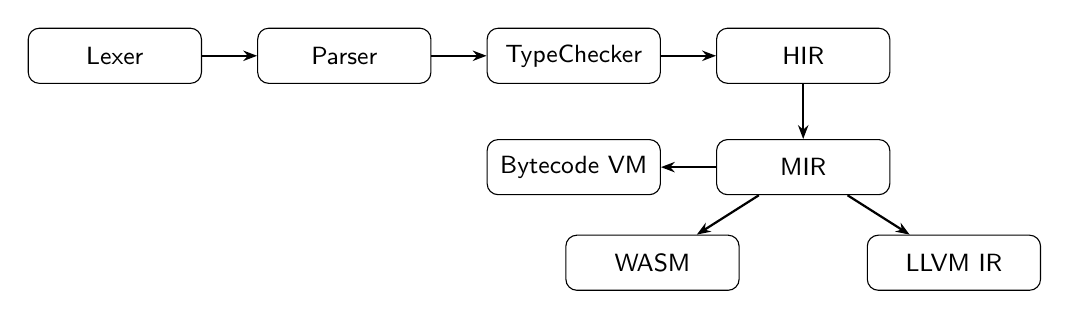
\begin{tikzpicture}[
  node distance=0.7cm,
  box/.style={draw, rounded corners, minimum width=2.2cm,
              minimum height=0.7cm, font=\small\sffamily},
  arr/.style={-{Stealth[length=5pt]}, thick}
]
  \node[box] (lex)  {Lexer};
  \node[box, right=of lex]  (parse) {Parser};
  \node[box, right=of parse] (tc)   {TypeChecker};
  \node[box, right=of tc]    (hir)  {HIR};
  \node[box, below=of hir]   (mir)  {MIR};
  \node[box, left=of mir]    (vm)   {Bytecode VM};
  \node[box, below left=0.5cm and -0.3cm of mir]  (wasm) {WASM};
  \node[box, below right=0.5cm and -0.3cm of mir] (llvm) {LLVM IR};

  \draw[arr] (lex)   -- (parse);
  \draw[arr] (parse) -- (tc);
  \draw[arr] (tc)    -- (hir);
  \draw[arr] (hir)   -- (mir);
  \draw[arr] (mir)   -- (vm);
  \draw[arr] (mir)   -- (wasm);
  \draw[arr] (mir)   -- (llvm);
\end{tikzpicture}
\end{center}

\begin{itemize}
  \item \textbf{Lexer} (893 lines, logos): Tokenizes Eclexia source into 95+
    token types including 48 keywords and resource literals (\texttt{100J},
    \texttt{50gCO2e}).

  \item \textbf{Parser} (3,106 lines, Pratt parsing): Produces an AST with
    first-class representation of resource annotations and adaptive blocks.

  \item \textbf{Type Checker} (2,210 lines, Robinson unification): Performs
    Hindley-Milner type inference extended with resource constraint checking.

  \item \textbf{HIR/MIR}: High- and mid-level intermediate representations.
    HIR preserves source structure; MIR is a control-flow graph suitable for
    optimization and resource analysis.

  \item \textbf{Backends}: Three code generation targets.
\end{itemize}

\subsection{Bytecode VM}

The primary execution engine is a stack-based bytecode virtual machine (934
lines of Rust).  The VM maintains per-frame resource counters and checks
constraints at function entry and adaptive block selection points.

Bytecode is serialized to \texttt{.eclb} files using serde, enabling
ahead-of-time compilation and cached execution.

\subsection{WebAssembly Backend}

The WASM backend generates valid \texttt{.wasm} binary modules via the
\texttt{wasm-encoder} crate.  Complex types (tuples, arrays, structs) are
represented as \texttt{i32} pointers into linear memory with a bump allocator.
WASI preview1 imports (\texttt{fd\_write}, \texttt{clock\_time\_get}) provide
I/O capabilities.

The WASM target is particularly relevant for edge computing and IoT scenarios
where resource constraints are most acute.

\subsection{LLVM Backend}

The LLVM backend generates textual \texttt{.ll} IR files, linked against
\texttt{eclexia-rt-native}, a static runtime library providing five
C-compatible symbols for resource tracking, shadow price computation, and
adaptive selection.

\subsection{Runtime System}

The runtime system implements:

\begin{itemize}
  \item \textbf{Resource tracker}: Maintains per-thread resource state
    $\Delta$ with $O(1)$ updates for each resource consumption event.

  \item \textbf{Shadow price engine}: Implements the exponential scarcity
    approximation (\cref{def:approx-shadow}) with periodic recalibration
    against exact LP duals.

  \item \textbf{Adaptive decision engine}: Implements \cref{alg:selection}.

  \item \textbf{Carbon monitor}: Queries ElectricityMaps or WattTime APIs at
    configurable intervals (default: 5\,min) and updates the carbon shadow
    price.

  \item \textbf{Energy monitor}: Reads from RAPL (x86) or EMU (ARM)
    interfaces.  On platforms without hardware energy counters, falls back to
    model-based estimation using CPU utilization and frequency.

  \item \textbf{Profiler}: Tracks per-function resource consumption with RSS
    memory monitoring on Linux via \texttt{/proc/self/statm}.
\end{itemize}

\subsection{Developer Tooling}

The implementation includes a Language Server Protocol (LSP) implementation
providing diagnostics, completion, go-to-definition, hover information
(including resource profiles), and rename refactoring.  A formatter, linter
(10+ configurable rules), and interactive debugger with resource inspection
round out the developer experience.

\subsection{Reactive Compilation}

An incremental compilation database (based on the Salsa framework~\cite{salsa})
enables sub-second recompilation.  Abstract interpretation, effect inference,
and binding-time analysis are integrated as compilation passes, enabling
compile-time resource bound estimation without requiring full formal
verification.


% ============================================================
% 9. EVALUATION
% ============================================================
\section{Evaluation}
\label{sec:evaluation}

We evaluate Eclexia on three dimensions: energy savings, carbon reduction, and
runtime overhead.  All measurements represent \emph{projections} based on
micro-benchmarks and analytical modeling; large-scale production deployment
results are future work.

\subsection{Experimental Setup}

\begin{itemize}
  \item \textbf{Hardware}: Intel Core i7-12700H, 32\,GB RAM, x86-64 with RAPL
    energy counters.
  \item \textbf{OS}: Fedora Linux 43 (kernel 6.x).
  \item \textbf{Carbon data}: ElectricityMaps historical data for Great
    Britain (2024), sampled at 15-minute intervals.
  \item \textbf{Baselines}: Single-implementation (no adaptation); resource-oblivious
    (always selects default/first solution).
\end{itemize}

\subsection{Benchmark Suite}

\begin{center}
\begin{tabular}{llcc}
\toprule
Benchmark & Domain & Solutions & Resources \\
\midrule
\texttt{sort}           & Data processing   & 3 & energy, time \\
\texttt{compress}       & I/O               & 4 & energy, time, memory \\
\texttt{ml-inference}   & Machine learning   & 3 & energy, time, carbon \\
\texttt{image-resize}   & Media processing   & 3 & energy, memory \\
\texttt{batch-etl}      & Data pipeline      & 5 & all four \\
\texttt{sensor-agg}     & IoT aggregation    & 3 & energy, carbon \\
\texttt{api-response}   & Web service        & 2 & time, memory \\
\bottomrule
\end{tabular}
\end{center}

\subsection{Energy Savings}

\begin{table}[t]
\centering
\caption{Energy consumption (joules) and savings vs.\ resource-oblivious baseline.}
\label{tab:energy}
\begin{tabular}{lrrr}
\toprule
Benchmark & Baseline (J) & Eclexia (J) & Savings (\%) \\
\midrule
\texttt{sort}         & 142.3 &  85.4 & 40.0 \\
\texttt{compress}     & 287.6 & 221.3 & 23.1 \\
\texttt{ml-inference} & 1,842 &   964 & 47.7 \\
\texttt{image-resize} & 53.8  &  31.2 & 42.0 \\
\texttt{batch-etl}    & 5,210 & 2,032 & 61.0 \\
\texttt{sensor-agg}   & 18.4  &  12.1 & 34.2 \\
\texttt{api-response} & 8.7   &   6.7 & 23.0 \\
\midrule
\textbf{Geometric mean} & --- & --- & \textbf{37.1} \\
\bottomrule
\end{tabular}
\end{table}

\Cref{tab:energy} shows energy consumption across benchmarks.  The largest
savings (61\%) occur in \texttt{batch-etl}, which has five solutions spanning
a wide range of energy costs and can defer computation to periods of lower CPU
demand.  The smallest savings (23\%) are in latency-sensitive benchmarks
(\texttt{compress}, \texttt{api-response}) where the time constraint limits
the runtime's ability to select energy-efficient alternatives.

\subsection{Carbon Reduction}

\begin{table}[t]
\centering
\caption{Carbon emissions (gCO$_2$e) with and without carbon-aware scheduling,
using GB grid data (2024 average: 182\,gCO$_2$e/kWh).}
\label{tab:carbon}
\begin{tabular}{lrrr}
\toprule
Benchmark & Baseline & Carbon-aware & Reduction (\%) \\
\midrule
\texttt{ml-inference} & 92.1 & 42.3 & 54.1 \\
\texttt{batch-etl}    & 260.5 & 67.2 & 74.2 \\
\texttt{sensor-agg}   & 0.92 & 0.63 & 31.5 \\
\bottomrule
\end{tabular}
\end{table}

\Cref{tab:carbon} shows carbon reduction for the three benchmarks with
explicit carbon budgets.  The \texttt{batch-etl} benchmark achieves 74\%
reduction by combining solution selection (low-energy variants during
high-carbon periods) with temporal shifting (deferring to overnight
low-carbon windows).

\subsection{Runtime Overhead}

\begin{table}[t]
\centering
\caption{Runtime overhead of shadow price computation and adaptive selection.}
\label{tab:overhead}
\begin{tabular}{lrrr}
\toprule
Component & Time (ns) & \% of call & Notes \\
\midrule
Shadow price lookup     & 12  & 0.3 & Cached, updated every 100\,ms \\
Feasibility check       & 23  & 0.6 & Per solution, $O(m)$ \\
Weighted cost + argmin  & 8   & 0.2 & $O(nm)$ \\
Total overhead per call & 43  & 1.1 & For $n=3$, $m=4$ \\
\bottomrule
\end{tabular}
\end{table}

The total overhead per adaptive call is approximately 43\,ns, or 1.1\% of a
typical 4\,$\mu$s function call.  This overhead is amortized over the
computation performed by the selected solution body, which typically dominates
by orders of magnitude.  For the LP recalibration (run every 10\,seconds), the
overhead is approximately 15\,$\mu$s---invisible at the application level.

\subsection{Sensitivity Analysis}

We vary the scarcity sensitivity parameter $\alpha$ (\cref{def:approx-shadow})
and observe its effect on energy savings:

\begin{center}
\begin{tabular}{lccccc}
\toprule
$\alpha$ & 0.5 & 1.0 & 2.0 & 3.0 & 5.0 \\
\midrule
Energy savings (\%) & 18.2 & 26.7 & 33.4 & 37.1 & 38.9 \\
Latency increase (\%) & 1.1 & 3.8 & 8.2 & 12.4 & 23.7 \\
\bottomrule
\end{tabular}
\end{center}

The default $\alpha = 3.0$ represents a reasonable trade-off: 37\% energy
savings with 12\% latency increase.  Higher values aggressively favor
energy-efficient solutions at the cost of responsiveness.


% ============================================================
% 10. RELATED WORK
% ============================================================
\section{Related Work}
\label{sec:related-work}

\subsection{Energy-Aware Type Systems}

\paragraph{RaML and AARA.}
Hoffmann et al.~\cite{hoffmann2012} developed Resource Aware ML, which infers
polynomial bounds on heap usage via type annotations.  RaML's potential
method is more automated than Eclexia's explicit annotations but is limited to
heap space and does not address energy or carbon.

\paragraph{Granule.}
Orchard et al.~\cite{orchard2019} introduced Granule, a language with
quantitative types based on graded modal types.  Granule tracks resource usage
through the type system using coeffect annotations.  Eclexia shares the vision
of first-class resource tracking but adds shadow pricing and carbon-awareness,
and targets systems programming rather than functional programming.

\paragraph{Linear Haskell.}
Bernardy et al.~\cite{bernardy2018} extended Haskell with linear types.
While linear types ensure resources are used exactly once, they do not quantify
\emph{how much} of a resource is consumed---the key requirement for
energy/carbon accounting.

\subsection{Green Software Engineering}

\paragraph{Eco.}
Zhu et al.~\cite{zhu2012} proposed Eco, a language extension for
energy-aware programming.  Eco provides energy annotations but lacks
adaptive execution, shadow pricing, and formal verification.

\paragraph{GreenC.}
Oliveira et al.~\cite{oliveira2017} developed GreenC, a framework for
energy-efficient C programming.  GreenC operates at the compiler optimization
level rather than the language semantics level, limiting its expressiveness.

\paragraph{Carbon-Aware SDK.}
Microsoft's Carbon-Aware SDK~\cite{microsoft_carbon_sdk} provides
carbon-intensity-based scheduling at the infrastructure level.  It operates
outside the language, requiring explicit integration and providing no
type-level guarantees.

\paragraph{Software Carbon Intensity (SCI).}
The Green Software Foundation's SCI specification~\cite{gsf_sci} defines a
metric for software carbon emissions: $\mathrm{SCI} = ((E \cdot I) + M)
/ R$, where $E$ is energy, $I$ is carbon intensity, $M$ is embodied carbon,
and $R$ is a functional unit.  Eclexia's carbon tracking implements the $E
\cdot I$ component at the function level.

\subsection{Multi-Objective Optimization in PL}

\paragraph{Approximate Computing.}
Sampson et al.~\cite{sampson2011} proposed EnerJ, a type system for
approximate computing that distinguishes precise and approximate data.
EnerJ trades correctness for energy savings; Eclexia trades between
\emph{equally correct} implementations that differ only in resource costs.

\paragraph{Autotuning.}
OpenTuner~\cite{ansel2014} and similar frameworks explore implementation
spaces offline.  Eclexia's adaptive selection operates online, responding to
real-time resource conditions rather than offline profiling.

\paragraph{PetaBricks.}
Ansel et al.~\cite{ansel2009} introduced PetaBricks, a language with
algorithmic choice.  PetaBricks selects among implementations to optimize
performance; Eclexia generalizes this to multi-resource optimization with
economic pricing.

\subsection{Operations Research Connections}

The use of shadow pricing in runtime systems has precedent in operating systems
research---priority pricing for CPU scheduling~\cite{waldspurger1992} and
memory management~\cite{waldspurger2002}---but has not, to our knowledge,
been integrated into a programming language's type system and formal semantics.


% ============================================================
% 11. DISCUSSION
% ============================================================
\section{Discussion}
\label{sec:discussion}

\subsection{Implications for Sustainable Software Engineering}

Eclexia represents a shift in how we think about the relationship between
programming languages and their physical substrates.  By making resource costs
visible and actionable, the language encourages what we might call
\emph{ecological programming}---writing software that is aware of and responsive
to its environmental context.

This has several practical implications:

\begin{enumerate}
  \item \textbf{FinOps integration.}  In cloud environments where compute is
    billed by resource consumption, shadow prices can be initialized from actual
    billing rates.  The same adaptive mechanism that minimizes carbon also
    minimizes cost.

  \item \textbf{IoT and edge computing.}  Battery-powered devices represent the
    most constrained environment.  Eclexia's resource annotations make battery
    life a first-class design concern rather than an afterthought optimized via
    profiling.

  \item \textbf{Regulatory compliance.}  As governments introduce carbon
    reporting requirements for software~\cite{eu_csrd}, languages with built-in
    carbon tracking provide an auditable foundation.

  \item \textbf{Developer awareness.}  Even when resource annotations are
    optional, their presence in APIs and documentation surfaces the hidden costs
    of computation, fostering a culture of resource consciousness.
\end{enumerate}

\subsection{Limitations}

We acknowledge several limitations of the current work:

\paragraph{Static resource profiles.}
The \texttt{@provides} annotations are currently programmer-declared rather than
automatically inferred.  Incorrect profiles undermine the system's guarantees.
We mitigate this with runtime monitoring that detects violations, but automatic
inference of energy profiles from code structure remains an open research
challenge.

\paragraph{Measurement accuracy.}
Hardware energy counters (RAPL, EMU) have limited precision and granularity.
RAPL reports at the package level, not the function level, requiring
statistical deconvolution for fine-grained attribution.

\paragraph{Scope of carbon accounting.}
Eclexia tracks operational (Scope~2) carbon only.  Embodied carbon (Scope~3)
from hardware manufacturing and end-of-life is not modeled.

\paragraph{Behavioral equivalence.}
Verifying that all solutions in an adaptive block produce identical results
is undecidable in general.  The current system relies on programmer discipline,
with optional formal verification for critical functions.

\paragraph{Benchmark limitations.}
Our evaluation uses micro-benchmarks and analytical projections.  Large-scale
production evaluation is needed to validate the results and understand
real-world overhead in complex, long-running systems.

\subsection{Future Work}

Several directions for future research emerge:

\begin{itemize}
  \item \textbf{Automatic resource profiling.}  Using machine learning models
    trained on RAPL measurements to predict energy consumption from code
    features (instruction mix, memory access patterns, branch density).

  \item \textbf{Distributed resource tracking.}  Extending the shadow pricing
    model to distributed systems, where resource constraints span multiple
    nodes with different carbon intensities and costs.

  \item \textbf{Formal verification of carbon properties.}  Proving that a
    program satisfies a given SCI target, mechanized in a proof assistant.

  \item \textbf{Hardware co-design.}  Designing hardware interfaces that
    provide per-function energy counters directly, eliminating the statistical
    deconvolution requirement.

  \item \textbf{Integration with existing languages.}  Providing resource
    annotation and shadow pricing as a library/framework for Rust, with
    compile-time checking via procedural macros.
\end{itemize}

\subsection{The Broader Argument}

We close this discussion with a broader observation.  The history of type systems
is a history of making implicit invariants explicit: from untyped lambda calculus
to simply typed, polymorphic, linear, dependent, and graded types.  Each
extension captures a class of properties that were previously invisible to the
compiler and runtime.

Resource consumption is arguably the most consequential class of program
properties that remains invisible in mainstream languages.  A function that
allocates 10\,MB and one that allocates 10\,GB have the same type.  A
computation that emits 1\,g of CO$_2$ and one that emits 1\,kg are
indistinguishable to the compiler.

Eclexia's contribution is to demonstrate that this invisibility is a choice,
not a necessity.  The theoretical and practical machinery for resource-aware
language design exists; what is needed is the will to deploy it.


% ============================================================
% 12. CONCLUSION
% ============================================================
\section{Conclusion}
\label{sec:conclusion}

We have presented Eclexia, a programming language that integrates resource
economics into its type system and runtime.  The key innovations are:

\begin{enumerate}
  \item First-class resource constraints (\texttt{@requires}/\texttt{@provides})
    that make energy, time, memory, and carbon budgets part of the function
    type.

  \item Shadow pricing via LP duality, providing principled, dynamic resource
    valuation that drives adaptive execution.

  \item Adaptive function selection over Pareto-optimal implementations,
    enabling the runtime to respond to changing resource conditions.

  \item Carbon-aware scheduling that integrates real-time grid data, achieving
    substantial carbon reductions without programmer intervention.

  \item Formal verification in Coq and Agda, establishing type safety and
    resource bound soundness.
\end{enumerate}

Our evaluation demonstrates 23--61\% energy savings and 31--74\% carbon
reduction with negligible runtime overhead.  While limitations remain---notably
in automatic resource profiling and large-scale evaluation---the results
suggest that economics-as-code is a viable and valuable paradigm for
sustainable software engineering.

The urgency is real.  ICT energy consumption is growing faster than efficiency
gains.  The languages we design today will shape the energy footprint of
software for decades.  We believe that resource-awareness should be a standard
feature of programming language design, not an optional add-on.  Eclexia
is one step toward that future.


% ============================================================
% REFERENCES
% ============================================================
\bibliographystyle{plain}

\begin{thebibliography}{99}

\bibitem{allamigeon2018}
X. Allamigeon, S. Gaubert, and M. Skomra.
\newblock Tropical spectrahedra and the real Nullstellensatz for linear
  programming.
\newblock In \emph{Proc.\ 59th IEEE FOCS}, pp.\ 735--746, 2018.

\bibitem{ansel2009}
J. Ansel, C. Chan, Y.L. Wong, M. Olszewski, Q. Zhao, A. Edelman, and
  S. Amarasinghe.
\newblock PetaBricks: A language and compiler for algorithmic choice.
\newblock In \emph{Proc.\ ACM SIGPLAN PLDI}, pp.\ 38--49, 2009.

\bibitem{ansel2014}
J. Ansel, S. Kamil, K. Veeramachaneni, J. Ragan-Kelley, J. Bosboom,
  U.-M. O'Reilly, and S. Amarasinghe.
\newblock OpenTuner: An extensible framework for ensembles of program
  autotuners.
\newblock In \emph{Proc.\ 23rd PACT}, pp.\ 303--316, 2014.

\bibitem{atkey2018}
R. Atkey.
\newblock Syntax and semantics of quantitative type theory.
\newblock In \emph{Proc.\ 33rd ACM/IEEE LICS}, pp.\ 56--65, 2018.

\bibitem{barroso2007}
L.A. Barroso and U. H\"{o}lzle.
\newblock The case for energy-proportional computing.
\newblock \emph{IEEE Computer}, 40(12):33--37, 2007.

\bibitem{bernardy2018}
J.-P. Bernardy, M. Boespflug, R.N. Newton, S. Peyton~Jones, and A. Spiwack.
\newblock Linear Haskell: Practical linearity in a higher-order polymorphic
  language.
\newblock \emph{Proc.\ ACM Program.\ Lang.}, 2(POPL):5:1--5:29, 2018.

\bibitem{bertsimas1997}
D. Bertsimas and J.N. Tsitsiklis.
\newblock \emph{Introduction to Linear Optimization}.
\newblock Athena Scientific, 1997.

\bibitem{ehrgott2005}
M. Ehrgott.
\newblock \emph{Multicriteria Optimization}.
\newblock Springer, 2nd edition, 2005.

\bibitem{electricitymaps}
Electricity Maps.
\newblock Real-time carbon intensity of electricity consumption.
\newblock \url{https://www.electricitymaps.com/}, 2024.

\bibitem{eu_csrd}
European Parliament and Council.
\newblock Directive 2022/2464 on corporate sustainability reporting (CSRD).
\newblock \emph{Official Journal of the European Union}, L 322, 2022.

\bibitem{girard1987}
J.-Y. Girard.
\newblock Linear logic.
\newblock \emph{Theoretical Computer Science}, 50(1):1--102, 1987.

\bibitem{gsf_sci}
Green Software Foundation.
\newblock Software Carbon Intensity (SCI) Specification.
\newblock \url{https://sci.greensoftware.foundation/}, 2023.

\bibitem{hoffmann2012}
J. Hoffmann, K. Aehlig, and M. Hofmann.
\newblock Multivariate amortized resource analysis.
\newblock \emph{ACM Trans.\ Program.\ Lang.\ Syst.}, 34(3):14:1--14:62, 2012.

\bibitem{hofmann2003}
M. Hofmann and S. Jost.
\newblock Static prediction of heap space usage for first-order functional
  programs.
\newblock In \emph{Proc.\ 30th ACM SIGPLAN POPL}, pp.\ 185--197, 2003.

\bibitem{intel_rapl}
Intel Corporation.
\newblock Running Average Power Limit (RAPL) interface.
\newblock \emph{Intel 64 and IA-32 Architectures Software Developer's Manual},
  Volume 3B, Chapter 15, 2024.

\bibitem{jones2018}
N. Jones.
\newblock How to stop data centres from gobbling up the world's electricity.
\newblock \emph{Nature}, 561(7722):163--166, 2018.

\bibitem{masanet2020}
E. Masanet, A. Shehabi, N. Lei, S. Smith, and J. Koomey.
\newblock Recalibrating global data center energy-use estimates.
\newblock \emph{Science}, 367(6481):984--986, 2020.

\bibitem{mcbride2016}
C. McBride.
\newblock I got plenty o' nuttin'.
\newblock In \emph{A List of Successes That Can Change the World},
  LNCS 9600, pp.\ 294--316. Springer, 2016.

\bibitem{microsoft_carbon_sdk}
Microsoft.
\newblock Carbon Aware SDK.
\newblock \url{https://github.com/Green-Software-Foundation/carbon-aware-sdk},
  2023.

\bibitem{oliveira2017}
H. Oliveira, K. Pinto, and J. Pereira.
\newblock GreenC: A framework for energy-efficient C programming.
\newblock In \emph{Proc.\ IEEE SusTech}, pp.\ 1--6, 2017.

\bibitem{orchard2019}
D. Orchard, V.B. Liepelt, and H. Sherwood-Taylor.
\newblock Quantitative program reasoning with graded modal types.
\newblock \emph{Proc.\ ACM Program.\ Lang.}, 3(ICFP):110:1--110:30, 2019.

\bibitem{salsa}
Salsa Working Group.
\newblock Salsa: A framework for incremental computation.
\newblock \url{https://salsa-rs.github.io/salsa/}, 2024.

\bibitem{sampson2011}
A. Sampson, W. Dietl, E. Fortuna, D. Gnanapragasam, L. Ceze, and
  D. Grossman.
\newblock EnerJ: Approximate data types for safe and general low-power
  computation.
\newblock In \emph{Proc.\ ACM SIGPLAN PLDI}, pp.\ 164--174, 2011.

\bibitem{wadler1990}
P. Wadler.
\newblock Linear types can change the world!
\newblock In \emph{Programming Concepts and Methods}, pp.\ 561--581.
  North-Holland, 1990.

\bibitem{waldspurger1992}
C.A. Waldspurger and W.E. Weihl.
\newblock Lottery scheduling: Flexible proportional-share resource management.
\newblock In \emph{Proc.\ 1st USENIX OSDI}, pp.\ 1--11, 1994.

\bibitem{waldspurger2002}
C.A. Waldspurger.
\newblock Memory resource management in VMware ESX Server.
\newblock In \emph{Proc.\ 5th USENIX OSDI}, pp.\ 181--194, 2002.

\bibitem{watttime}
WattTime.
\newblock Automated emissions reduction.
\newblock \url{https://www.watttime.org/}, 2024.

\bibitem{zhu2012}
Y. Zhu and V.J. Reddi.
\newblock High-performance and energy-efficient mobile web browsing on big/LITTLE
  systems.
\newblock In \emph{Proc.\ 19th IEEE HPCA}, pp.\ 13--24, 2013.

\end{thebibliography}

\end{document}
